\chapter{Money and Inflation}\label{chp:mpin}
\hypertarget{inflation}{}

\textbf{Tools:} The quantity theory; central bank balance sheet; open market operations.

\textbf{Key Words:} Price level; inflation; quantity theory; velocity; hyperinflation.

\textbf{Big Ideas:}
\vspace{-0.1in}
\begin{itemize}
\item Inflation is the growth rate of the price level,
which is typically measured by a price index.
\item The quantity theory links the money supply with the price level and output.
In the long run, an increase in the money supply results in an increase in the price level (inflation).
\item Hyperinflation refers to an inflation rate of 100\% per year or more.
Hyperinflations follow a standard pattern: government deficits are financed with money,
which produces inflation.
\end{itemize}
\rule{\textwidth}{1pt}

Inflation is the rate of growth of the price level,
typically measured by a price index.
Milton Friedman, winner of the 1976 Nobel Prize in economics, once
said: ``Inflation is always and everywhere a monetary phenomenon.
To control inflation, you need to control the money supply.''
Friedman believed what he said, but he also enjoyed
thumbing his nose at the popular Keynesian theory of the 1960s,
in which inflation was the result of excess demand for goods.

Was Friedman right?
We consider his claim in the context of big inflations (``hyperinflations''):
episodes of annual inflation exceeding 100 percent per year.
Although extreme, big inflations are a recurring phenomenon
and a wonderful laboratory for
studying inflation more generally.
In these situations (but not necessarily in others),
money growth is present,
but it's invariably connected to government deficits.
The keys to stopping a big inflation, then, are to
balance the government's budget and prevent the central bank from expanding the money supply.


\section{The quantity theory}

Friedman's claim about inflation is based on a theory that is
several centuries old: the {\it quantity theory of
money\/}. Like a lot of good theory, it's based on an analogy. Think
for a moment about the effect of a two-for-one stock split on the
price of a stock. If it's now selling for 100, then you'd probably
expect it to sell for 50 after the split. (This wouldn't be true if
the split were a signal of some new information about the firm,
but let's assume it's not.) The point is that the value of a firm's
total stock of equity shouldn't depend on anything as arbitrary as
the number of shares.

Now suppose we do the same thing with money.  This is
unrealistically simple, but makes the point effectively. Suppose that the
government replaced every dollar with two ``new dollars,''
marked so we could tell the difference between old and new notes. Then
you'd expect that new dollars would be worth half as much
as old dollars. That is, you'd expect prices of goods and services
quoted in new dollars to be twice as high as prices quoted in old
dollars. In short, changes in the quantity of money in circulation
(the ``money supply'') executed in this way will be associated with
proportionate changes in prices, with no effect on output.  Why the
latter? Because output is determined by productivity and inputs, and
we wouldn't expect either one to be influenced by the number of
pieces of paper used to make transactions.

Of course the world is more complicated than this, and monetary
policy consists of more than just currency exchanges, but some of
the same reasoning applies more generally (we'll look at some data
shortly). The quantity theory is the result of two ideas:  that
money is not fundamental (pieces of paper don't change the
productivity of the US or Chinese economies), and that its
usefulness is in executing transactions.  Let's start with the
latter. In all developed economies, transactions consist of
exchanges of goods and services for money. If we approximate the volume of
transactions in an economy by nominal GDP, then we have
$M=PY$, where $Y$ is real GDP and $P$ is a measure of the
price level such as the GDP deflator. This isn't quite right yet. A
dollar can be used to execute several different transactions in a
given year.
To take this into account, we use
%
\begin{eqnarray}
    M V  &\equiv&  P Y,
    \label{eq:quantity_theory}
\end{eqnarray}
%
where $V$ is the \textit{velocity} of money: the number of times a
dollar is used to execute transactions in a given year.

At this level of generality,
equation (\ref{eq:quantity_theory}) is a tautology:
For any data we collect on $M$, $P$, and $Y$,
we simply choose $V$ to make the equation hold.
What gives the equation content is Friedman's
assumption that velocity $V$ is (at least approximately)
constant.  This implies that increases in $M$ are associated with
proportionate increases in $PY$.
We add one further assumption to get Friedman's connection between
money and prices:
that real GDP is determined by the productivity and inputs of the economy,
and is not affected by the amount of money in circulation.
We can change that later, but it seems like a good place to start.


The same theory explains inflation if we express it in growth rates.
As with growth accounting, we focus on \hyperref[sec:growth_math_cc]{continuously compounded growth rates} where the growth rate of a variable $X$ is
$ \gamma_X = \ln X_t - \ln X_{t-1}$.
In logs, equation (\ref{eq:quantity_theory}) and its first difference are:
%
\begin{eqnarray*}
    \ln M_t + \ln V_t &=& \ln P_t + \ln Y_t \\
    (\ln M_t - \ln M_{t-1})  + (\ln V_t - \ln V_{t-1})
                 &=& (\ln P_t - \ln P_{t-1}) + (\ln Y_t - \ln Y_{t-1})\\
    \gamma_M  + \gamma_V &=&  \pi + \gamma_Y ,
\end{eqnarray*}
%
where $\pi = \gamma_P $ is the inflation rate
(rate of growth of the price level).
If we assume that velocity is constant,
\begin{eqnarray}
    \gamma_M   &=&  \pi + \gamma_Y ,
    \label{eq:quantity_theory-growth}
\end{eqnarray}
and changes in the growth rate of money are associated
with changes in the growth rate of inflation and output.
The second assumption is that the growth rate of money does not influence
output, so changes in money growth translate one-for-one
into changes in inflation.
That's Friedman's argument, which depends on these two assumptions.


\section{Evidence}

It's not that easy to check the second assumption, but we can
check the first (constant velocity) by looking at the components of
equation (\ref{eq:quantity_theory}).
They imply that velocity is constant and that movements in the price
level $P$ mirror those in $M/Y$.
We can see both in Figure~\ref{fig:quantity_long} for the US.
(Money here is \href{http://research.stlouisfed.org/fred2/series/M2}{M2}.)
The figure suggests that the theory is a reasonable approximation of the data, at least
over the last fifty years or so.
The two increasing lines ($P$ and $M/Y$)
show some short-run differences, but their movements are similar.
Velocity itself wiggles around a little, but is not
much different now than it was in 1960.
%
\begin{figure}[h]
    \caption{The quantity theory in the long run.}
    \label{fig:quantity_long}
    \centering
    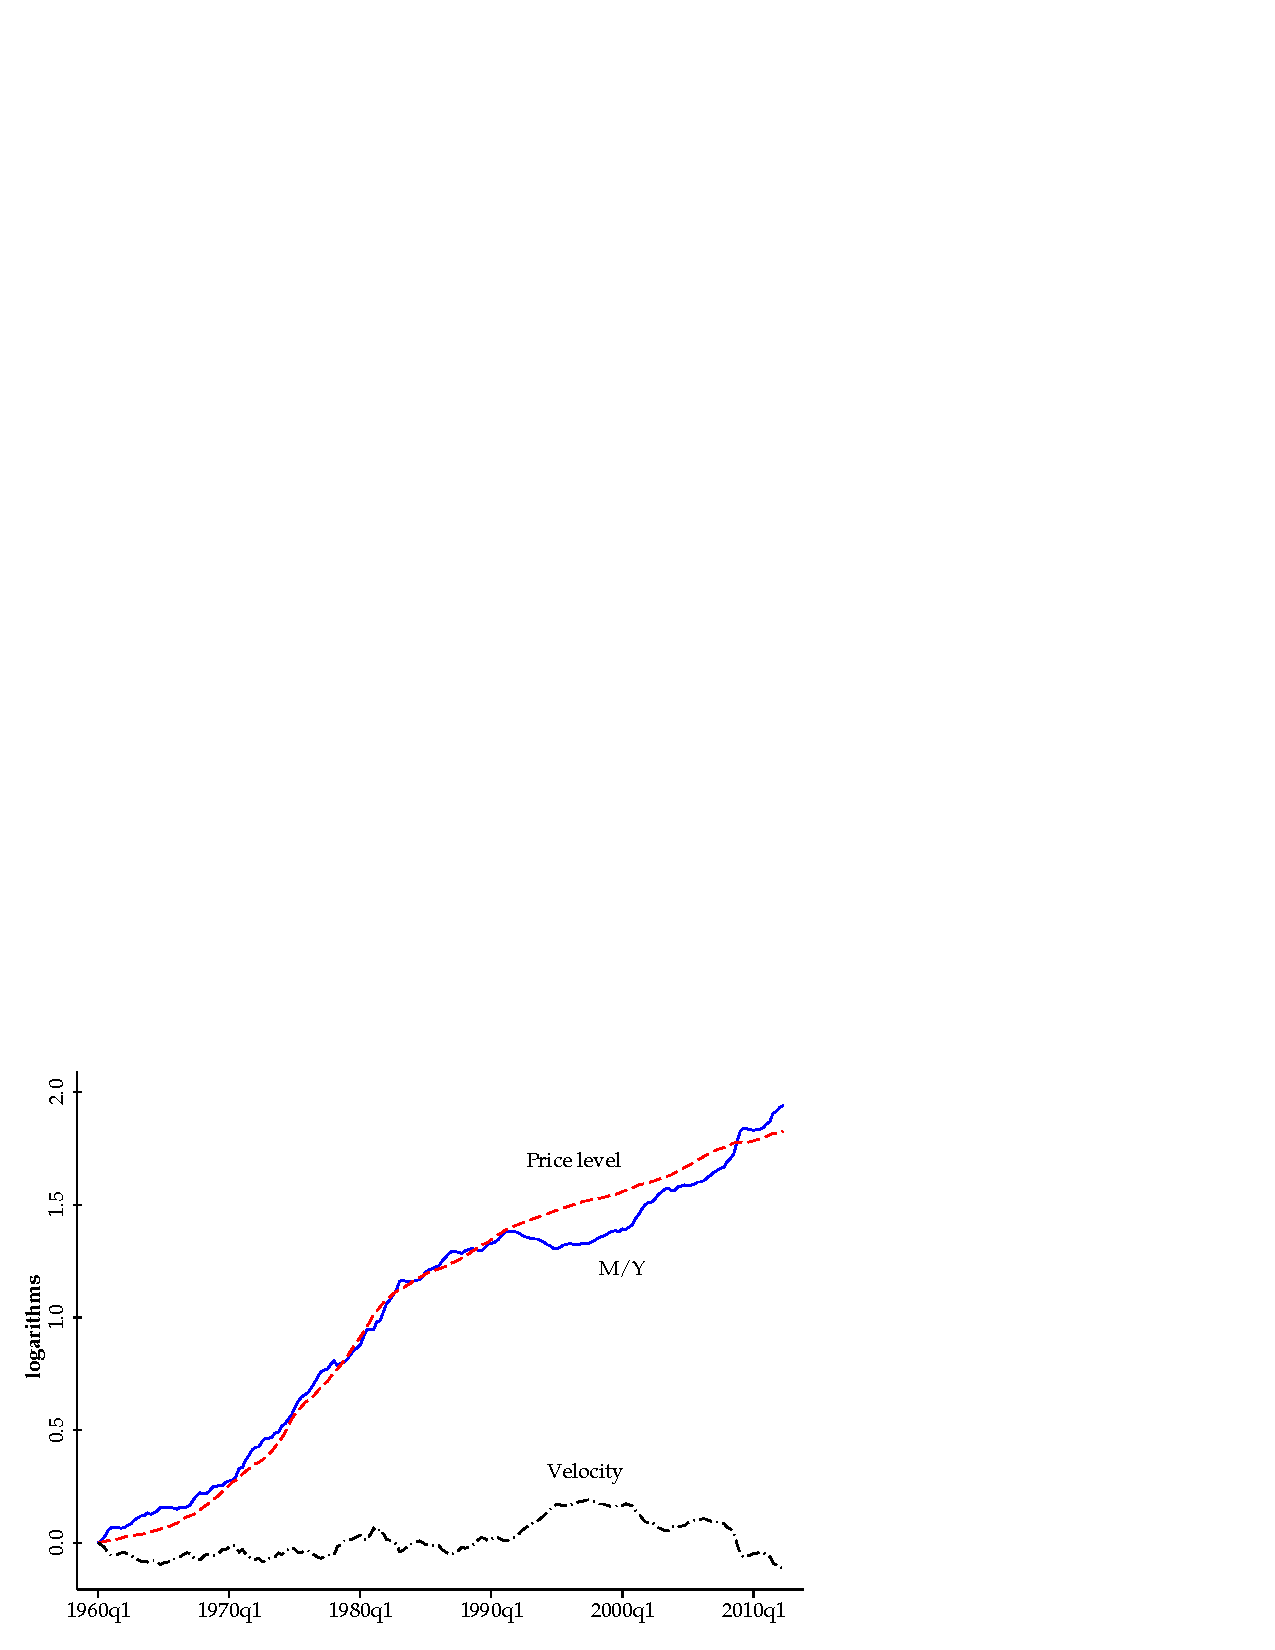
\includegraphics[width=0.8\textwidth]{Figures/long.pdf}
\end{figure}
%

The evidence for short-run changes is much different.
When we look at deviations from trend (Figure~\ref{fig:quantity_short}), movements in prices are only loosely related to movements in money, and
velocity has as much short-run volatility as the stock of money.
%We'll discuss the short run later in the course, where we try to
%figure out the impact of monetary policy on real output,
%inflation, and interest rates.

\begin{figure}[h]
    \caption{The quantity theory in the short run.}
    \label{fig:quantity_short}
    \centering
    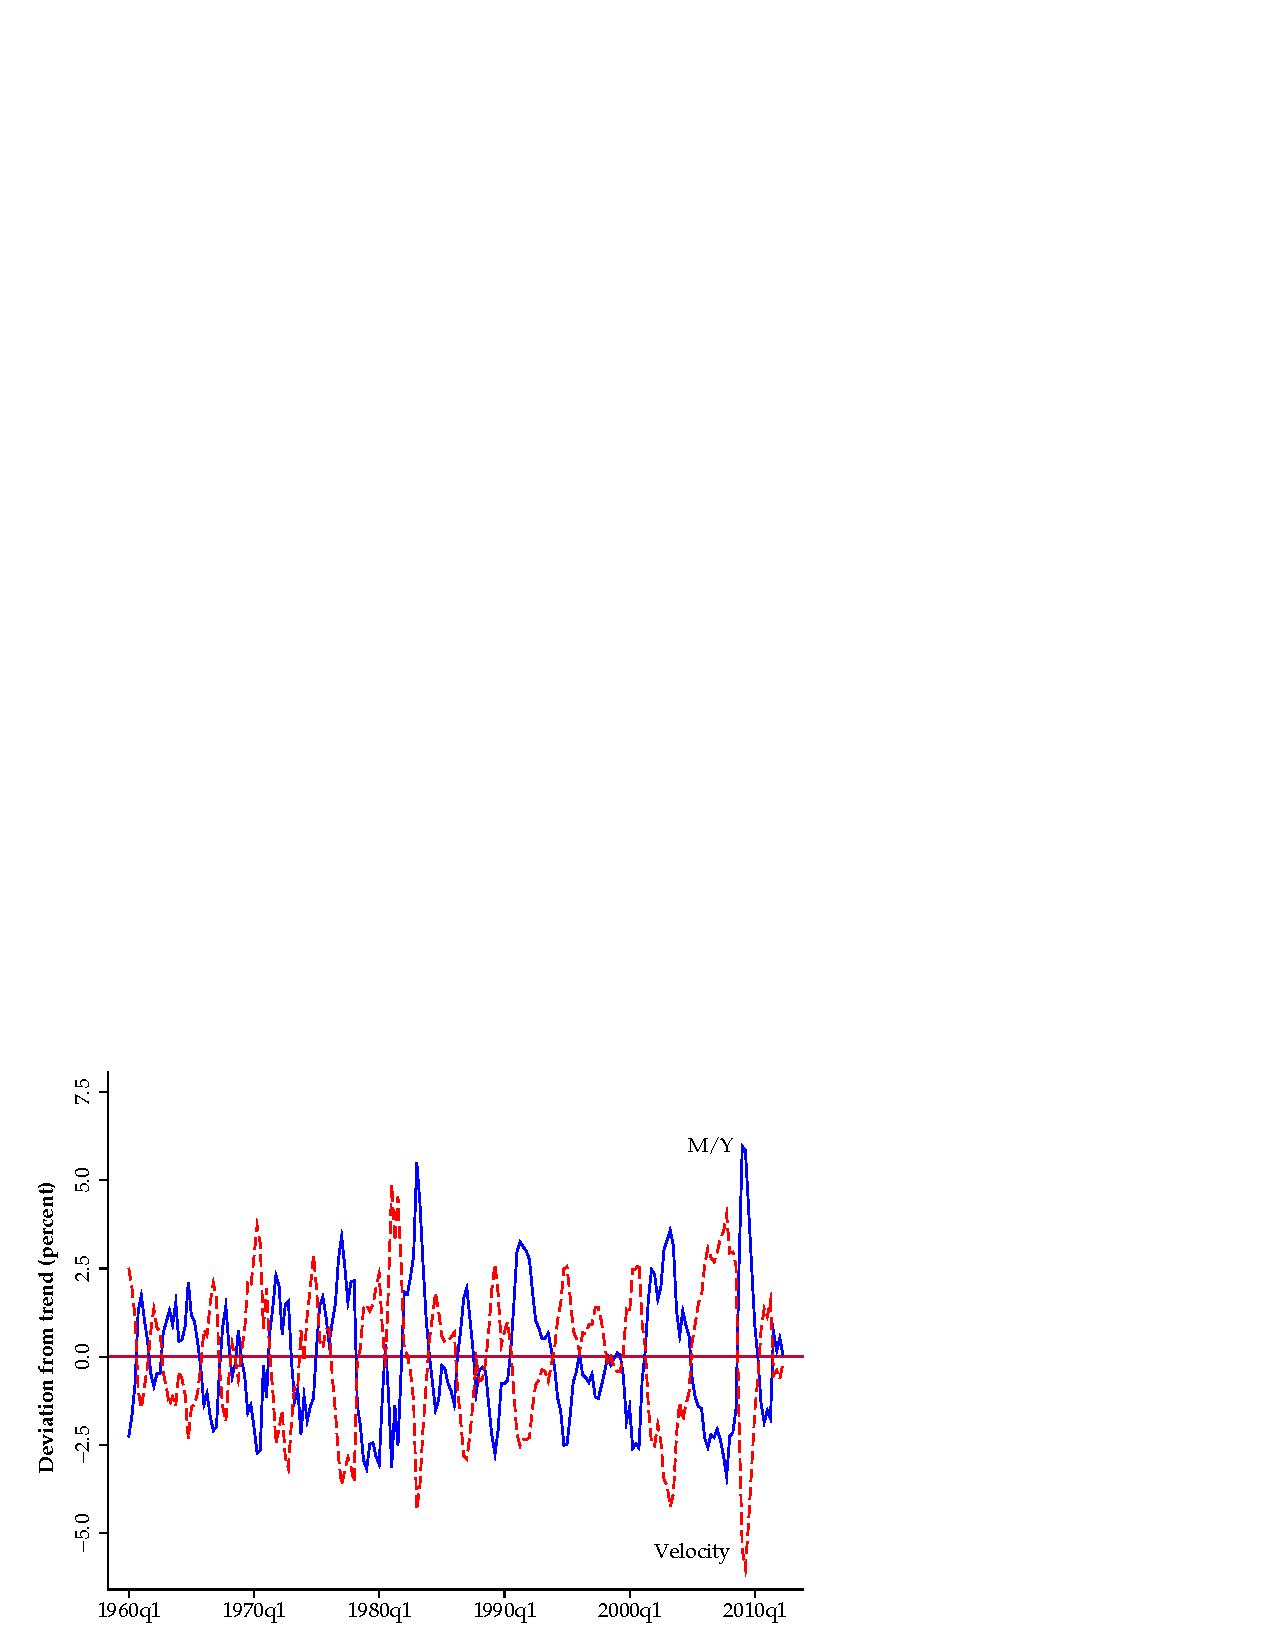
\includegraphics[width=0.8\textwidth]{Figures/short_1.pdf}
\end{figure}


\section{Changing the money supply}

Currency is a liability of the government,
which can (and does) change the quantity in circulation.
To see how this works, it's helpful to take a
step back and consider the broader issue of government debt.
We can divide the government's debt management into two
related pieces.
The first piece is the size of the debt.
Measured in units of currency (dollars, say, or pesos),
the debt changes over time as the government runs surpluses
or deficits.
Mathematically, we might write:
\begin{eqnarray*}
    \mbox{Debt}_{t} &=& \mbox{Debt}_{t-1} + \mbox{Deficit}_t .
\end{eqnarray*}
This is an example of a government budget constraint, something
we'll see more of later on.
The second piece is the composition of the debt.
In practice, governments have many different liabilities,
but for the purposes of this discussion, let us say, it has two:
government bonds and money (currency).
In both theory and practice,
these two pieces are typically separate,
with the treasury issuing bonds to cover the entire debt
and the monetary authority (central bank) buying back
some of these bonds and issuing money in return.

Day-to-day monetary policy in most countries consists of what we term
{\it open-market operations\/}:  purchases or sales of
government debt (bonds).
At any point in time, the treasury's balance sheet looks
something like:
%
\begin{center}
\begin{tabular}{lr|lr}
%\multicolumn{4}{l}{Treasury} \\
Assets\phantom{ities}  &\phantom{100}&  Liabilities \\
\hline
& & Bonds & 200
\end{tabular}
\end{center}
%
and the central bank's looks like:
%
\begin{center}
\begin{tabular}{lr|lr}
Assets\phantom{ities}  &&  Liabilities \\
\hline
Bonds &  100 & Money & 100
\end{tabular}
\end{center}
%
If it seems strange to treat money as a liability of the
central bank (isn't money an asset?),
think of it as a bond with the unusual
feature that its nominal interest rate is zero.
That's what it is, which makes it a good deal for the borrower.

An open-market purchase of bonds results in an increase
in bonds held by the central bank and an equal increase in its
monetary liability.
For example, a purchase of 20 worth, of bonds would change its
balance sheet to:
%
\begin{center}
\begin{tabular}{lr|lr}
Assets\phantom{ities}  &&  Liabilities \\
\hline
Bonds &  120 & Money & 120
\end{tabular}
\end{center}
%
The result is an increase in the amount of money in private hands,
since the private sector (the other side of this transaction)
has reduced its holdings of government bonds
and increased its holdings of money.
Similarly, an open-market sale of bonds would reduce the amount of money in
private hands.

The question we're leading up to is why money growth is so high
in countries with big inflations.
Why does the central bank keep issuing money?


\section{Big Inflations}

If inflation is as easily cured as Friedman suggests
(``control the money supply''),
why do big inflations happen?
People who live through such
episodes describe them as traumatic; they spend an hour or more
every day converting cash into anything with stable value:  real estate,
cars, foreign assets.
The economy is usually a mess, but whether that is cause or effect is
hard to say.
But if big inflations are so painful, why do governments let them happen?
The problem, typically, starts with a government deficit.
A political impasse makes it nearly impossible to reduce the deficit.
Given the government's budget constraint, it must then issue debt.
There is apparently no shortage of ready buyers of US debt
(ditto other developed countries),
but the same can't be said for every country.
If no one will buy its debt,
the remaining option is to finance the deficit with money
(read: oblige the central bank to purchase bonds
from the treasury).
In short, when the government can't
pay its bills in any other way, it pays them with money, which is
easy enough to print.
The effect of this, of course, is inflation.

Nobel Prize-winner Thomas Sargent and his co-author, Neil Wallace,
have shown that even a central bank that aims for low inflation will fail
 if the government issues debt without end. Think of the problem as
 a version of the \hyperref[sec:time_cons]{time-consistency problem} discussed in Chapter \ref{chp:insp}. If everyone knows that the
 central bank eventually will be compelled to print money to avoid outright default by the government, inflation expectations
 will rise today despite the central bank's caution. The key is
 that the bank cannot credibly commit to limit future money creation, while
 expectations of the future drives price setting today.

The conventional solution to ending a big inflation has two parts.  The
first is fiscal discipline: Balance the government budget.  The
second is monetary discipline: Separate the central bank
from the treasury and tell the bank that its job is to maintain
price stability. Though there are many of fine points --- how quickly must
the deficit be eliminated?  should the IMF supply short-term
financing?  --- the outlines of the problem and its solution
are clear.
%Brazil managed to bring inflation under control by tightening its budget.
Going back to Friedman's quote: Inflation may be a monetary phenomenon,
but the trouble often starts with fiscal policy and the political situation that led to it.

For someone operating an international business,
the thing to remember is that ``big inflations''
are relatively common.
What do you do if you're hit with one?
You'll probably find that the
most important thing you can do is streamline your cash management.
If you can reduce the payment
terms from (say) 60 days to 30 days, you increase your ``real'' revenue substantially.
You may also find that big inflations lead to policies --- such as price controls and capital controls --- that make life more complicated.
Finally, you may find that your financial statements
are highly misleading, since they measure performance in terms of the local
currency, the value of which is changing rapidly.
For a US subsidiary, high inflation triggers a change
in the rules for translating financial entries into dollars for tax and reporting purposes.

\section{Inflation and interest rates}

The interest rates we typically use are nominal: They tell us how much money we get in the future
for a given investment of money today.
Since inflation measures the change in the value
of money, it shows up in interest rates.
More concretely, we would say that the nominal interest
rate equals the real interest rate (the interest rate
adjusted for inflation) plus \textit{expected} inflation:
\begin{eqnarray}
    i_t &=& r_t + \pi_t^e .
    \label{eq:mpin_fisher}
\end{eqnarray}
For a given real interest rate $r$,
an increase in expected inflation raises the nominal interest rate
one for one.


Here is the deeper explanation behind equation (\ref{eq:mpin_fisher}).
Consider a one-year interest rate on a Treasury bill.
The rate tells us how many dollars (say)
we get in one year for a given payment of dollars today.
For example, if a 12-month treasury bill has a price
of \$96.15, its annualized yield is the value of $i$ that solves
%
\begin{eqnarray}
    96.15 &=& \frac{100}{1+i_t}.
    \label{eq:nominal_yield}
\end{eqnarray}
%
In this case, $i_t = 4$ percent.  Thus, each dollar invested today gives us
1.04 dollars in 12 months.
We refer to $i_t$ as the  {\it nominal rate of interest\/} --- nominal because its refers to payments of currency.

For many purposes, we'd like to know not only the dollar yield, but
also how much 1.04 dollars will buy when we get it.  If we expect
the inflation rate to be 3 percent a year, then we'd guess that three quarters of the
interest will be eaten up by inflation.  The investment gains
us only about one percent in terms of purchasing power.
We refer to the increase in purchasing power as the
{\it real rate of interest\/} --- real because it refers to the
quantity of real consumption it finances.
That gives us equation (\ref{eq:mpin_fisher}).


We can show this more formally
by translating the words into equations more carefully.
We have just argued that investors are interested not in the money the
bond is a claim to, but in what that money will buy. If by ``what
that money will buy,'' we mean the basket of goods used to construct
the CPI, we can define the real interest rate $r$ as
%
\begin{eqnarray*}
    (96.15/P_t) &=& \frac{100/ P_{t+1}}{1+r_t},
\end{eqnarray*}
%
where $P_{t}$ is the CPI index in year $t$ and $P_{t+1}$ is the
expected value of the same index in year $t+1$. What we are doing
here is expressing the current bond price, measured in terms of what
it will buy, as the discounted value of the principal, also measured
in terms of what it will buy. Doing a little algebra, we find
%
\begin{eqnarray*}
    (1+r_t)(P_{t+1}/P_{t}) &=& 100/96.15.
\end{eqnarray*}
%
Then, equation (\ref{eq:nominal_yield}) tells us that the real and
nominal interest rates are related by
\begin{eqnarray*}
    1 + i_t   &=& (1+r_t)(1+\pi_{t}^e),
\end{eqnarray*}
where $(P_{t+1}-P_t)/P_t $ is the expected inflation rate between
$t$ (now) and $t+1$ (a year from now). Since the product
$r_{t}\pi_{t}^e$ is a small number when expected inflation is low, it follows that
\begin{eqnarray*}
    i_t  &\approx&  r_t + \pi_{t}^e, \ \mbox{for \ small \ values \ of \ $r$ and $\pi_{t}^e$},
\end{eqnarray*}
where $\approx$ means ``equals approximately.''
If we're careful about timing, we see that all three variables
are comparisons between now and one year from now.
Inflation is, therefore, typically understood to be
expected inflation, since we don't know what inflation
will be when we buy the bond.
In principle, we could also take into account the risk
inherent in inflation --- but we won't.


Now that we're done with definitions, we can ask how inflation
affects nominal interest rates.
In principle, either component (the real rate or expected inflation)
can change the nominal interest rate.
In practice, we typically find that in periods of
high and variable inflation,
the inflation component dominates.
This is approximately true of the US, where high-inflation periods
(the 1970s and early 1980s)
are high-interest-rate periods, too.
It's even more evident in countries with very high inflation rates.


\section{Velocity reconsidered}

In very-high-inflation environments,
people often find that that the inflation rate accelerates
quickly, often far exceeding the rate of money growth.
One factor here is velocity, which typically
rises sharply with inflation.
Why?
Because inflation (and nominal interest) is effectively a tax on holding money:
The higher the tax, the less money you hold.
During big inflations,
people spend money as soon as they get it, because its
value falls by the minute.
It's common, for example, for people to buy groceries
and gasoline as soon as they get their paychecks;
if they wait even a day or two, their purchasing power falls.

If velocity $V$ rises with inflation, then we can reconsider
\begin{eqnarray}
    \gamma_M + \gamma_V  &=&  \pi + \gamma_Y .
\end{eqnarray}
If $\gamma_Y$ is approximately constant,
then an increase in money growth not only
produces inflation directly, but
its impact is also magnified by the increase in the
interest rate, which increases velocity ($\gamma_V > 0$).
Similarly, when hyperinflations are reversed,
we often see a larger drop in inflation
than in money growth, as velocity falls.


\section*{Executive summary}

\setlength{\leftmargini}{.5\oldleftmargini}
\begin{enumerate}
\item Over long periods of time, inflation is closely related to money growth.

%\item High inflation is usually associated with
%high (nominal) interest rates.

\item Extremely high rates of inflation are invariably associated with high rates of money growth.

\item High money growth is often the result of financing large fiscal deficits with money.
    The deficits, in turn, often reflect some kind of political gridlock.

\item High inflation is typically associated with high interest rates,
since investors demand higher yields to compensate for the loss of purchasing
power of the currency.
\end{enumerate}
\setlength{\leftmargini}{\oldleftmargini}

\section*{Review questions}

\setlength{\leftmargini}{.5\oldleftmargini}
\begin{enumerate}
\item Policy rule.  Friedman suggested that the Fed might do better to adopt
a rule in which it kept the growth rate of the money supply constant.
\begin{enumerate}
\item If the growth rate of real GDP is 3 percent, on average,
what growth rate of the money supply would deliver
average inflation of 2 percent?
\item What are the strengths and weaknesses of such a policy rule?
\end{enumerate}

Answer.
\begin{enumerate}
\item If velocity is constant, then
equation (\ref{eq:quantity_theory-growth}) gives us
a money growth rate of
\begin{eqnarray*}
    \gamma_M &=& \pi + \gamma_Y
            \;\;=\;\;  2 + 3 \;\;=\;\; 5.
\end{eqnarray*}
In words: Money growth accommodates inflation and economic growth.
\item Strengths: predictable, good average inflation performance,
avoid major policy mistakes.
Weakness: no room for policy to respond to current conditions.
Compare, for example, policy in the aggregate supply and demand model
(coming up).
\end{enumerate}


\item Central bank independence.
Why do many countries make central banks independent of the treasury?

Answer.  The idea is that monetary policy should focus on good long-term
performance and, to accomplish this, should be immune to
short-term political pressure.
With respect to hyperinflations,
you might argue that if the government does not have access to money finance,
it will be forced to confront its deficit issues earlier,
which is a good thing.



\item Zimbabwe.
Zimbabwe ended its hyperinflation by abandoning its currency.
Even official transactions were switched to either US dollars or
    South African rand.
    Does this seem like a good solution?
    Does it make sense for a country to abandon its currency?

Answer.  There's a long tradition of each country having its own currency,
but there's good reason to think at least some countries would be better
off using someone else's.
Zimbabwe has shown no ability to manage it99s own currency effectively,
so using another sounds like a move in the right direction.
There are other examples --- Panama and Colombia use the US dollar --- and perhaps there should be more.

\item Interest rates and inflation.  Go to
\href{http://research.stlouisfed.org/fred2/}{FRED} and find
the three-month treasury bill rate (TB3MS)
and the consumer price index (CPIAUCSL).
Manipulate them as needed and graph
the nominal interest rate and inflation rate together.
What do you see?

Answer.  Do it and see!

\end{enumerate}
\setlength{\leftmargini}{\oldleftmargini}


\section*{If you're looking for more}

Similar material is covered in most macroeconomics textbooks.
Wikipedia has a nice article on hyperinflation,
including a list of the biggest ones of all time.

Steve Hanke and Nicholas Krus survey the compete history of
hyperinflation in 
``\href{http://www.cato.org/publications/working-paper/world-hyperinflations}{World Hyperinflations}.''
Search:  ``hanke krus hyperinflation.''
Two really good (but more technical) pieces about specific episodes are 
Thomas Sargent, 
``\href{http://www.nber.org/chapters/c11452.pdf}{The ends of four big inflations},''
and Thomas Sargent and Joseph Zeira,
``\href{http://www.sciencedirect.com/science/article/pii/S1094202511000147}
{Israel 1983}.''


\section*{Symbols and data used in this chapter}

\begin{table}[H]
\centering
\caption{Symbol table.}
\begin{tabular*}{0.8\textwidth}{l@{\extracolsep{\fill}}l}
\toprule
Symbol & Definition\\
\midrule
$M$            &Money stock\\
$V$            &Velocity of money\\
$P$            &Price level\\
$Y$            &Real output or GDP\\
$\ln$        &Natural log\\
$\gamma_x$    &Continuously compounded growth rate of $x$\\
$\pi$         &Inflation ($= P$)\\
$\pi^{e}$    &Expected Inflation\\
$i$            &Nominal interest rate\\
$r$            &Real interest rate ($= i- \pi^e$)\\
\bottomrule
\end{tabular*}
\end{table}

\begin{table}[htb]
\centering
\caption{Data table.}
\begin{tabular*}{0.8\textwidth}{l@{\extracolsep{\fill}}l}
\toprule
Variable & Source\\
\midrule
Nominal GDP                    &GDP\\
M2 monetary aggregate        &M2SL\\
M2 velocity                    &M2V\\
Consumer Price Index        &CPIAUCSL\\
\bottomrule
\addlinespace
\end{tabular*}
\begin{minipage}{0.8\textwidth}
\footnotesize{To retrieve the data online, add the identifier from the source column to \url{http://research.stlouisfed.org/fred2/series/}.  For example, to retrieve nominal GDP, point your browser to \url{http://research.stlouisfed.org/fred2/series/GDP}}
\end{minipage}
\end{table}
